\newcommand{\dox}{\frac{\mathrm{d}}{\mathrm{d}x}}
\newcommand{\doxP}[1]{\dox\left({#1}\right)}
\newcommand{\lnp}[1]{\ln\left({#1}\right)}
\newcommand{\eqWithMsg}[1]{\overset{{#1}}{=\joinrel=}}
\newcommand{\longEqWithMsg}[1]{\xlongequal{\!{#1}\!}}
\newcommand{\tabspace}{\;\;\;} % VERY UGLY HACK
\newcommand{\xtabspace}{\tabspace\tabspace\tabspace\tabspace} % VERY UGLY HACK
\DeclareRobustCommand\iff{\;\Longleftrightarrow\;}


\section*{\S{6.6} Derivatives of Inverse Trigonometric Functions}
\begin{equation}
\begin{split}
    \doxP{\sin^{-1} x} = \frac{1}{\sqrt{1 - x^2}} \tabspace& \doxP{\csc^{-1} x} = -\frac{1}{x\sqrt{x^2 + 1}} \\\\
    \doxP{\cos^{-1} x} = \frac{1}{-\sqrt{1 - x^2}} \tabspace& \doxP{\sec^{-1} x} = -\frac{1}{x\sqrt{x^2 - 1}} \\\\
    \doxP{\tan^{-1} x} = \frac{1}{1 + x^2} \tabspace& \doxP{\cot^{-1} x} = -\frac{1}{1 + x^2}
\end{split}
\end{equation}

\section*{\S{6.6} Integrals of Inverse Trigonometric Functions}
\begin{equation}
\begin{split}
    \int \frac{1}{\sqrt{1 - x^2}} \;\mathrm{d}x &= \sin^{-1} x + C \\\\
    \int \frac{1}{x^2 + 1} \;\mathrm{d}x &= \tan^{-1} x + C \\\\
    \int \frac{1}{\sqrt{x^2 + a^2}} \;\mathrm{d}x &= \frac{1}{a}\tan^{-1}\left(\frac{x}{a}\right) + C
\end{split}
\end{equation}

\section*{\S{6.7} Hyperbolic Functions}
\begin{equation}
\begin{split}
    \sinh x = \frac{e^x - e^{-x}}{2} \tabspace& \csch x = \frac{1}{\sinh x} \\\\
    \cosh x = \frac{e^x + e^{-x}}{2} \tabspace& \sech x = \frac{1}{\cosh x} \\\\
    \tanh x = \frac{\sinh x}{\cosh x} \tabspace& \coth x = \frac{\cosh x}{\sinh x}
\end{split}
\end{equation}
\begin{center}
    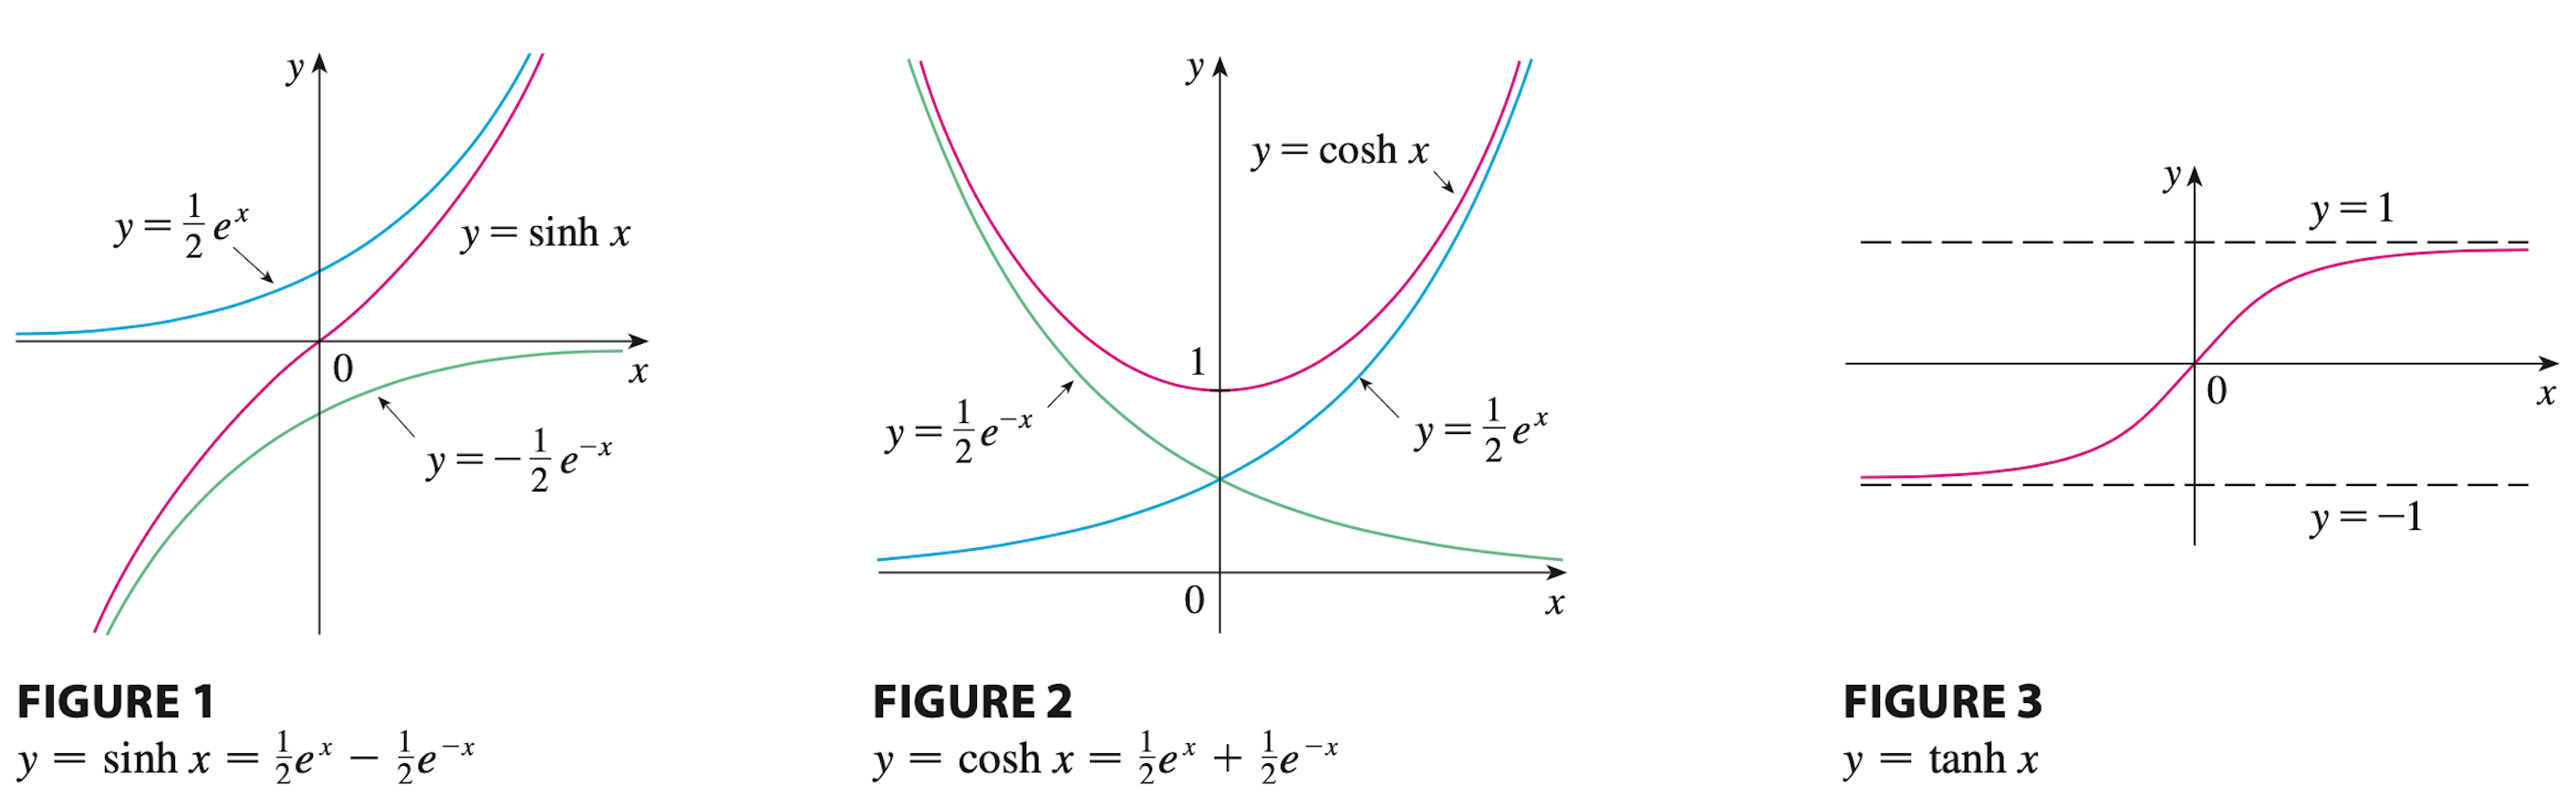
\includegraphics[width=1.0\linewidth]{../images/calc-textbook/6.7/2.png}
\end{center}

\section*{\S{6.7} Hyperbolic Function Identities}
\begin{equation}
\begin{split}
    \sinh(-x) = -\sinh(x) \xtabspace& \cosh(-x) = \cosh(x) \\\\
    \cosh^2 x - \sinh^2 x = 1  \xtabspace& 1 - \tanh^2 x = \sech^2 x\\\\
\end{split}
\end{equation}
\begin{equation}
\begin{split}
    \sinh(x + y) &= \sinh x \cosh y + \cosh x \sinh y \\\\
    \cosh(x + y) &= \cosh x \cosh y + \sinh x \sinh y
\end{split}
\end{equation}

\section*{\S{6.7} Hyperbolic Function Derivatives}
\begin{equation}
\begin{split}
    \doxP{\sinh x} = \cosh x \tabspace& \doxP{\csch x} = -\csch x \coth x \\\\
    \doxP{\cosh x} = \sinh x \tabspace& \doxP{\sech x} = -\sech x \tanh x \\\\
    \doxP{\tanh x} = \sec^2 x \tabspace& \doxP{\coth x} = -\csch^2 x
\end{split}
\end{equation}

\section*{\S{6.7} Inverse Hyperbolic Functions}
\begin{equation}
\begin{split}
    y = \sinh^{-1} x &\iff \sinh y = x\\
    \text{for all $y \geq 0$}\;\; y = \cosh^{-1} x &\iff \cosh y = x\\
    y = \tanh^{-1} x &\iff \tanh y = x
\end{split}
\;\;\;\left\{
\begin{array}{ll}
    \sinh^{-1} x = \ln\left( x + \sqrt{x^2 + 1} \right) \;\; x \in \mathbb{R} \\\\
    \cosh^{-1} x = \ln\left( x + \sqrt{x^2 - 1} \right) \;\; x \geq 1 \\\\
    \tanh^{-1} x = \frac{1}{2} \ln\left(\frac{x + 1}{1 - x}\right) \;\; -1 \leq x < 1
\end{array}
\right.
\end{equation}
\begin{center}
    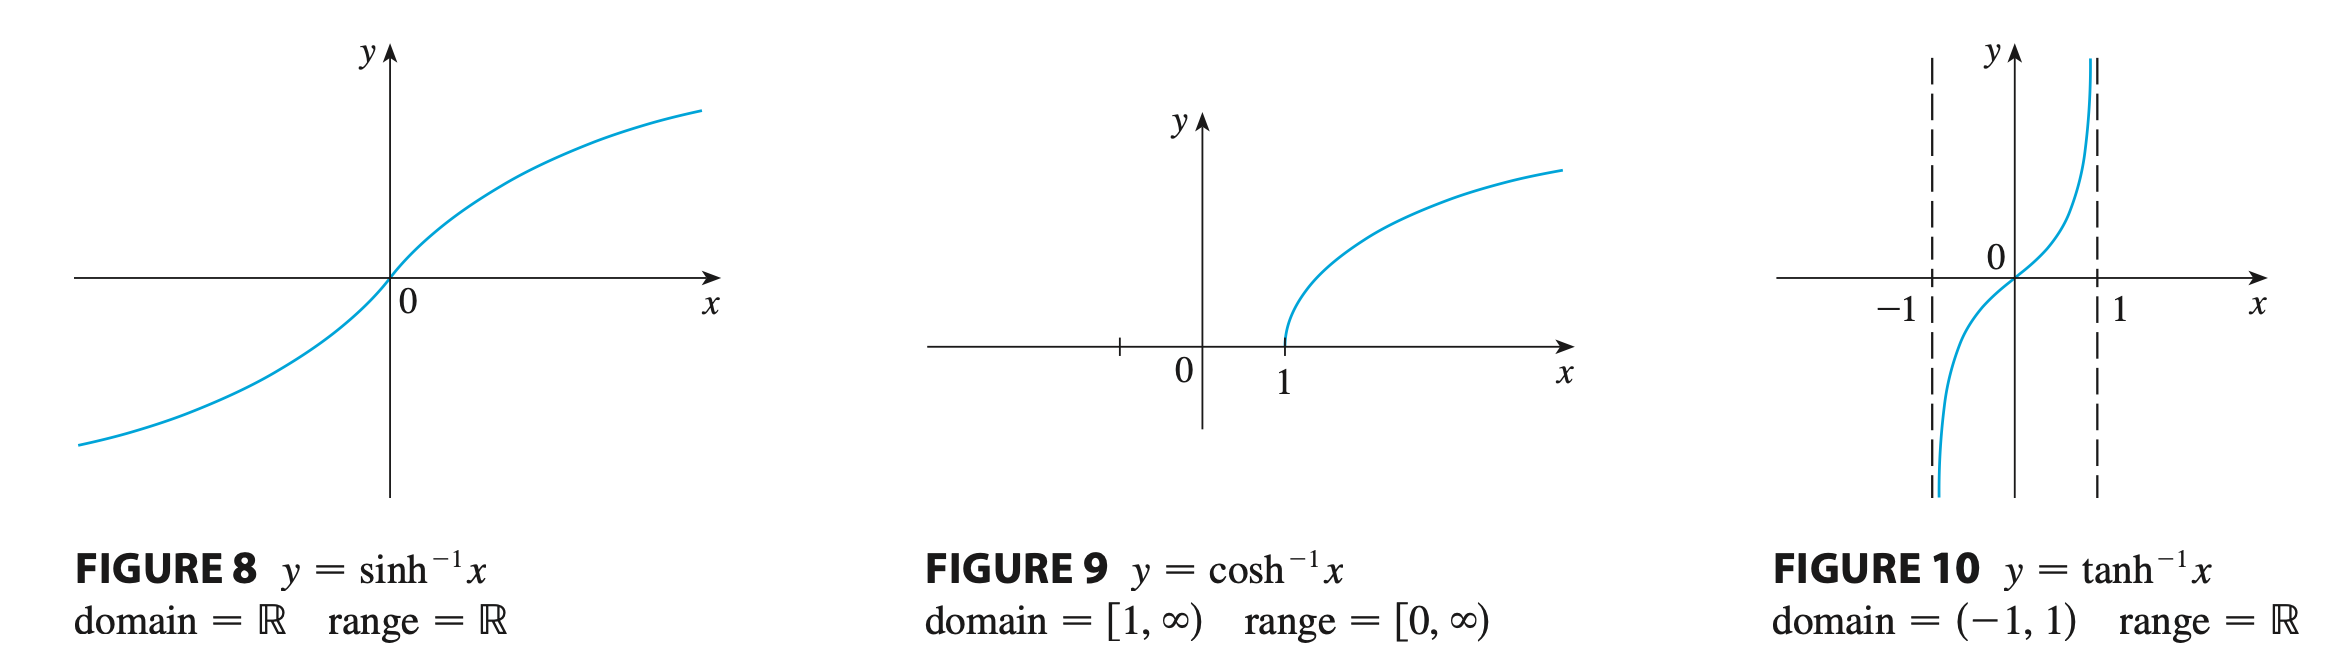
\includegraphics[width=1.0\linewidth]{../images/calc-textbook/6.7/6.png}
\end{center}

\section*{\S{6.7} Inverse Hyperbolic Function Derivatives}
\begin{equation}
\begin{split}
    \doxP{\sinh^{-1} x} = \frac{1}{\sqrt{1 + x^2}} \tabspace& \doxP{\csch^{-1} x} = -\frac{1}{|x| \sqrt{x^2 + 1}} \\\\
    \doxP{\cosh^{-1} x} = \frac{1}{\sqrt{x^2 - 1}} \tabspace& \doxP{\sech^{-1} x} = -\frac{1}{x\sqrt{1 - x^2}} \\\\
    \doxP{\tanh^{-1} x} = \frac{1}{1 - x^2} \tabspace& \doxP{\coth^{-1} x} = \frac{1}{1 - x^2}
\end{split}
\end{equation}